

Certain Atomify-commands can be added to the comments of a regular LAMMPS script
to modify properties of the GUI.
All these start with \keys{\texttt{\#}} so that LAMMPS ignores them as they are
interpreted as comments.
For instance, the color and size of the atoms can be set based on the type by
the command \keys{\texttt{\#/atom}}.
To set the color to white and radius to 2.0 for particle type 1,
the user can apply the command \keys{\texttt{\#/atom 1 2.0 \#ffffff}}.
Certain built-in atom types have default values and can be accessed with
\keys{\texttt{\#/atom 1 oxygen}} for simplicity.
The initial camera position can also be set similarily.
For a full list of the available commands, see the Atomify
documentation\citep{atomifydocumentation}.

Atomify provides live visualization of particles in a simulation in its 3D view. 
The particles can be colored based on any produced per-atom quantity in LAMMPS such as
atom type, velocity, force or a variable formula.
The coloring scheme can be changed while the simulation is running by hovering
the mouse cursor over groups in the dashboard.
Light colors and strength can also be changed in the dashboard.
This will be described in further detail in the following section.

It is possible to organize particles in groups and regions in LAMMPS.
These are shown in the dashboard in Atomify, which also provides controls to
highlight or hide specific groups or regions.
To highlight a group or region, the user only needs to hover the name in the
dashboard.
The visibility icon can be clicked to hide a group or region.

Parameters for rendering, such as the light strength,
attenuation, and color can be modified in the Rendering tab of the dashboard.
See the above section about the script editor for information about how to
modify the color of the particles.

In LAMMPS, computes are computations performed on a group of atoms.
Variables are user defined expressions which can be used to combine values in
calculations.
Once defined in a LAMMPS script, these can be plotted as a function of time in
Atomify.
This is done by clicking the name of the variable or compute in the simulation
tab.
We will explore plots in further detail in the following section.

Any operation that is applied to the system in a LAMMPS timestep or minimization
step is called a ``fix''.
These fixes are defined in the LAMMPS script using the ``fix'' keyword.
Atomify registers all defined fixes and lists these in the dashboard.

In LAMMPS, computes are physical quantities calculated based on the running
simulation, such as energy, temperature and stress.
% TODO better word for measures?
These are typically macroscopic measures derived from the microscopic
interactions between the atoms.
Computes and variables are shown in the Atomify dashboard,
along with information about the regions, groups and fixes as shown in figure
\ref{fig:dashboard}.

\begin{figure}
	\centering
	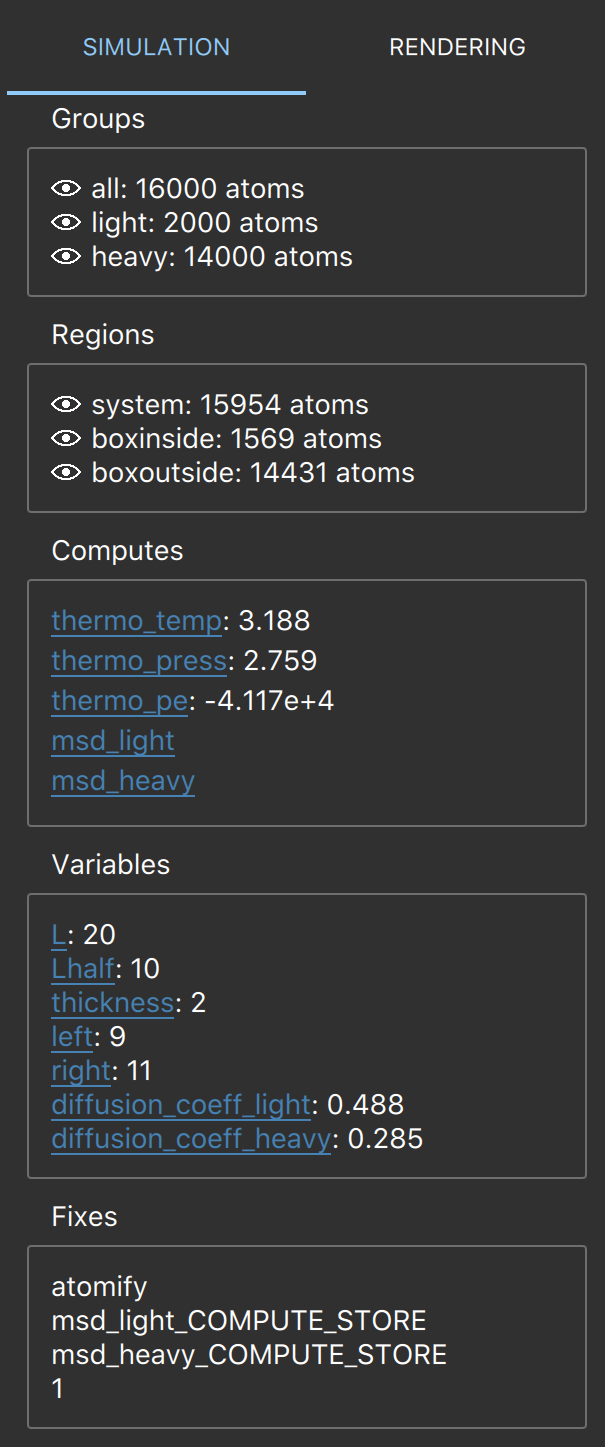
\includegraphics[width=0.3\textwidth]{dashboard.png}
	\caption{Dashboard}
	\label{fig:dashboard}
\end{figure}

Computes can be plotted as a function of time and visualized while the 
simulation is running.
Quantities that are measured per atom can be plotted in a histogram or a 2D
average for each region.
Atomify provides live visualization of the compute values using various plotting
techniques.
For instance, the temperature of the simulated system can be plotted as a
function of time as seen in figure \ref{fig:temperature}.

% \begin{figure}
% 	\centering
% 	\includegraphics[width=0.45\textwidth]{figures/temperature.png}
% 	\caption{Atomify can visualize computes defined in LAMMPS. 
%     Here the temperature is plotted as a function of time.}
% 	\label{fig:temperature}
% \end{figure}
